%%%%%%%%%%%%%%%%%%%%%%
%%%%%%%%%%%%%%%%%%%%%%
%
%                                        PRE-AMBLE
%
%%%%%%%%%%%%%%%%%%%%%%
%%%%%%%%%%%%%%%%%%%%%%

\documentclass[11pt]{amsart}

\setlength{\textwidth}{\paperwidth}
\addtolength{\textwidth}{-3in}
\calclayout

% LOAD PACKAGES--------------------------------------------

\usepackage{amsfonts, amsthm, amssymb, amsmath, stmaryrd, etoolbox}
\usepackage{comment}
\usepackage{mathtools}
\usepackage{graphicx,caption,subcaption}
\usepackage{todonotes}
\usepackage{xcolor}

\usepackage[inline]{enumitem}
\setlist{itemsep=0em, topsep=0em, parsep=0em}
\setlist[enumerate]{label=(\alph*)}

\usepackage{tikz}
\usepackage[all,2cell]{xy}
\usetikzlibrary{matrix,arrows,shapes,decorations.markings,decorations.pathreplacing}
\definecolor{rewritecolor}{rgb}{0,.9,1}
\tikzset{rewritenode/.style={shape=circle,fill=rewritecolor,scale=0.25,font=\Huge}}
\tikzset{RWopen/.style={shape=circle,draw=black,fill=white,scale=0.5,font=\Huge}}
\tikzset{RWclosed/.style={shape=circle,fill=black,scale=0.5,font=\Huge}}
\tikzset{CDnode/.style={shape=circle,fill=white,scale=.5}}
\tikzset{zxgreen/.style={shape=circle,draw,thick,fill=green}}
\tikzset{zxred/.style={shape=circle,draw,thick,fill=red}}
\tikzset{zxyellow/.style={shape=rectangle,draw,thick,fill=yellow}}
\tikzset{zxdiamond/.style={shape=diamond,fill=black,inner sep=2.75}}
\tikzset{zxopen/.style={shape=circle,draw,thick,inner sep=2pt}}
\tikzset{->-/.style={decoration={%
			markings,
			mark=at position .5 with {\arrow{>}}},postaction={decorate}}
}
\tikzset{->-pos/.style={decoration={%
			markings,
			mark=at position #1 with {\arrow{>}}},postaction={decorate}}
}

\usepackage{hyperref}
\definecolor{hyperrefcolor}{rgb}{0,0,0.7}
\hypersetup{colorlinks,linkcolor={hyperrefcolor},citecolor={hyperrefcolor},urlcolor={hyperrefcolor}}

%NEW COMMANDS---------------------------------------------

\newcommand{\RR}{\mathbb{R}}
\newcommand{\ZZ}{\mathbb{Z}}
\newcommand{\NN}{\mathbb{N}}
\newcommand{\QQ}{\mathbb{Q}}
\newcommand{\CC}{\mathbb{C}}
\renewcommand{\epsilon}{\varepsilon}
\newcommand{\DD}{\mathbb{D}}


\newcommand{\cl}[1]{\mathcal{#1}}
\newcommand{\scr}[1]{\mathscr{#1}}
\newcommand{\op}[1]{\operatorname{#1}}
\newcommand{\cat}[1]{\mathbf{#1}}
\newcommand{\dblcat}[1]{\mathbb{#1}}
\renewcommand{\t}[1]{\textup{#1}}

\newcommand{\from}{\colon}
\newcommand{\xto}[1]{\xrightarrow{#1}}
\newcommand{\sm}{\smallsetminus}
\newcommand{\tospan}{\xrightarrow{\mathit{sp}}}
\newcommand{\tocospan}{\xrightarrow{\mathit{csp}}}

%\newcommand{\diagram}[1]{\raisebox{-0.5\height}{\includegraphics{#1}}}

\newcommand{\bluebullet}{\textcolor{rewritecolor}{\bullet}}

%  macros for (co)span bicategories
\newcommand{\bispmap}[1]{\mathbf{Sp(#1)}}
\newcommand{\dblspmap}[1]{\mathbb{S}\mathbf{p(#1)}}
\newcommand{\bicspmap}[1]{\mathbf{Csp(#1)}}
\newcommand{\dblcspmap}[1]{\mathbb{C}\mathbf{sp(#1)}}
\newcommand{\bispsp}[1]{\mathbf{Sp(Sp(#1))}}
\newcommand{\dblspsp}[1]{\mathbb{S}\mathbf{p(Sp(#1))}}
\newcommand{\bicspcsp}[1]{\mathbf{Csp(Csp(#1))}}
\newcommand{\dblcspcsp}[1]{\mathbb{C}\mathbf{sp(Csp(#1))}}
\newcommand{\bimonspcsp}[1]{\mathbf{MonicSp(Csp(#1))}}
\newcommand{\dblmonspcsp}[1]{\mathbb{M}\mathbf{onicSp(Csp(#1))}}
\newcommand{\biepiccspsp}[1]{\mathbf{EpicCsp(Sp(#1))}}
\newcommand{\dblepiccspsp}[1]{\mathbb{E}\mathbf{picCsp(Sp(#1))}}
\newcommand{\bispcs}[1]{\mathbf{Sp}(\mathbf{Csp}(\mathbf{#1}))}

% defining arrow with a vertical line through it
\makeatletter
\def\slashedarrowfill@#1#2#3#4#5{%
	$\m@th\thickmuskip0mu\medmuskip\thickmuskip\thinmuskip\thickmuskip
	\relax#5#1\mkern-7mu%
	\cleaders\hbox{$#5\mkern-2mu#2\mkern-2mu$}\hfill
	\mathclap{#3}\mathclap{#2}%
	\cleaders\hbox{$#5\mkern-2mu#2\mkern-2mu$}\hfill
	\mkern-7mu#4$%
}
\def\rightslashedarrowfill@{%
	\slashedarrowfill@\relbar\relbar\mapstochar\rightarrow}
\newcommand{\xslashedrightarrow}[2][]{%
	\ext@arrow 0055{\rightslashedarrowfill@}{#1}{#2}}
\makeatother

\newcommand{\hto}{\xslashedrightarrow{}}


%DECLARE MATH OPERATORS----------------------------------

\DeclareMathOperator{\Hom}{Hom}
\DeclareMathOperator{\id}{id}
\DeclareMathOperator{\ob}{Ob}
\DeclareMathOperator{\arr}{arr}
\DeclareMathOperator{\im}{im}
\DeclareMathOperator{\Aut}{Aut}
\DeclareMathOperator{\Bij}{Bij}
\DeclareMathOperator{\Sub}{Sub}

%ENVIRONMENTS AND COUNTERS---------------------------------

\newtheorem{thm}{Theorem}[section]
\newtheorem{lem}[thm]{Lemma}
\newtheorem{prop}[thm]{Proposition}
\newtheorem{cor}[thm]{Corollary}

\theoremstyle{remark}
\newtheorem{remark}[thm]{Remark}
\newtheorem{notation}[thm]{Notation}

\theoremstyle{definition}
\newtheorem{ex}[thm]{Example} 
\newtheorem{defn}[thm]{Definition}

%\setcounter{tocdepth}{1} % Sets depth for table of contents. 

% FOR THIS PAPER ONLY

\newcommand{\zx}{_{\text{zx}}}
\newcommand{\bicat}[1]{\underline{\mathbf{#1}}}
\newcommand{\SpCspZX}{\cat{Sp}(\cat{Csp}(\cat{Graph}\downarrow S_{\text{zx}}))}
\newcommand{\zxGraphs}{\cat{Graph} \downarrow S_{\text{zx}}}

%%%%%%%%%%%%%%%%%%%%%%
%%%%%%%%%%%%%%%%%%%%%%
%%%%%%%%%%%%%%%%%%%%%%
%%%%%%%%%%%%%%%%%%%%%%
%
%BEGIN DOCUMENT
%
%%%%%%%%%%%%%%%%%%%%%%
%%%%%%%%%%%%%%%%%%%%%%
%%%%%%%%%%%%%%%%%%%%%%
%%%%%%%%%%%%%%%%%%%%%%

\begin{document}
	
%\tableofcontents

\begin{abstract}
	This paper presents a symmetric monoidal and compact closed bicategory that categorifies the zx-calculus developed by Coecke and Duncan.  The $1$-cells in this bicategory are certain graph morphisms that correspond to the string diagrams of the zx-calculus, while the $2$-cells are rewrite rules. To prove this category is symmetric monoidal, we use Shulman's technique involving symmetric monoidal double categories.  
\end{abstract}

\title{Categorifying the zx-calculus}
\author{Daniel Cicala}
\maketitle

%%%%%%%%%%%%%%%%%%%%%%
%%%%%%%%%%%%%%%%%%%%%%
% INTRODUCTION
\section{Introduction}
\label{sec:Introduction}
%%%%%%%%%%%%%%%%%%%%%%
%%%%%%%%%%%%%%%%%%%%%%

Compositionality is becoming increasingly recognized as a method to model complex systems.  The idea is that one can instead study smaller,simpler systems and ways of connecting them together.  The word \emph{compositionality} suggests that category theory can play a key role, and indeed it does.  Systems are morphisms and connections are morphism composition.   \todo{cite some examples here} 

This paper looks at one example of compositionality in action: the zx-calculus.  The backstory to this dates back to Penrose's tensor networks \cite{Penrose_NegDimTensors} and, more recently, to the relationship between graphical languages and monoidal categories explored by Joyal and Street as well as Selinger \cite{JoyalStreet_GeomTensorCalc,Selinger_GraphicsMonCats}.  Then Abramsky and Coecke took advantage of this relationship when they invented a categorical framework for quantum physics \cite{AbramCoecke_CatSemanticQuantum}.  So with a categorically oriented point of view, Coecke and Duncan \cite{CoeckeDuncan_QuantumObs} developed a diagrammatic language in which to reason about complementary quantum observables called the zx-calculus.   There are five basic diagrams, 
\[
	
\includegraphics{generater_wire}
	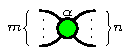
\includegraphics{generater_green_spider}
	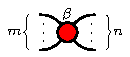
\includegraphics{generater_red_spider}
	
\includegraphics[]{generater_hadamard}
	
\includegraphics{generater_diamond}
\]
which can be combined in various ways to form larger, more complex diagrams.   Observe that these diagrams have dangling wires on the left and right.  Those on the left are to be thought of as inputs and those on the right as outputs.  Hence, these diagrams generate the morphisms of a dagger compact category $\cat{zx}$ whose objects are the non-negative integers whose meaning is number of inputs and outputs.

In this paper, we introduce a symmetric monoidal and compact closed (SMCC) bicategory $\bicat{zx}$ which categorifies $\cat{zx}$.  We begin Section \ref{sec:RewritingOpenGraphs} with a discussion of open graphs and constructing a SMCC bicategory $\cat{Rewrite}$ of ($0$-cells) non-negative integers, ($1$-cells) open graphs, and  ($2$-cells) rewrites of open graphs.  This bicategory is actually the $1$-full and $2$-full SMCC-bicategory of $\bispcs{Graph}$ which has ($0$-cells) graphs, ($1$-cells) cospans of graphs, and ($2$-cells) certain isomorphism classes of spans of cospans of graphs \cite{Cicala_SpansCospans, CicalaCourser_BicatSpansCospan}.   

After spending Section \ref{sec:ZxCalc} introducing the zx-calculus, we take Section \ref{sec:OpenGraphsOverSzx} to discuss `open graphs over $S\zx$'.  That is, we pick a graph $S\zx$
\[
	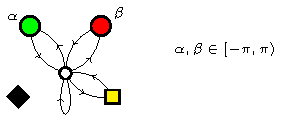
\includegraphics{graph_S_zx}
\]  
in such a way that graphs over $S\zx$, that is graph morphisms $G \to S\zx$ correspond exactly to the $zx$-morphisms.  This gives an SMCC bicategory that is analogous to $\bispcs{Graph}$. Namely, using the over category $\zxGraphs$, we look at $\bispcs{\zxGraphs}$ which has ($0$-cells) graphs over $S\zx$, ($1$-cells) cospans of graphs over $S\zx$, and ($2$-cells) certain isomorphism classes of spans of these cospans.  The parallel category to $\cat{Rewrite}$ is named $\cat{zxRewrite}$. To define this, we first introduce the functor
\[
	N\zx \from \cat{Set}_0 \to \zxGraphs
\]
on a skeleton of the category $\cat{Set}$.  Define $N\zx(X)$ to be the edgeless graph with nodes $X$ and is constant on the $S\zx$-node $
\begin{tikzpicture} \node [zxopen] at (0,0) {}; \end{tikzpicture}$.  This allows us to construct the SMCC sub-bicategory $\cat{zxRewrite}$ that is $1$-full and $2$-full on the $0$-cells of form $N\zx (X)$.  

Now, $\cat{zxRewrite}$ is a space in which we can generate SMCC sub-bicategories by choosing generating $1$-cells corresponding to the basic zx- calculus diagrams  and $2$-cells corresponding to the relations on $\cat{zx}$. In Section \ref{sec:zx categorified}, we introduce these $1$-cells and $2$-cells which present the SMCC bicategory $\bicat{zx}$.  After constructing $\bicat{zx}$, we immediately decategorify to an $1$-category $\operatorname{decat}(\bicat{zx})$ by identifying $1$-cells if there is a $2$-cell between them.  This seems asymmetrical, but dual nature of spans allows this to actually give an equivalence relation, not merely generate one.  Our main result is Theorem \ref{thm:equiv of zx cats} which constructs a dagger compact functor $\operatorname{decat}(\bicat{zx}) \to \cat{zx}$ that is an equivalence of categories.  

The author would like to thank his advisor John Baez for many helpful ideas and discussions that contributed to this paper.   

%%%%%%%%%%%%%%%%%%%%%%
%%%%%%%%%%%%%%%%%%%%%%
% A BICATEGY FOR REWRITING OPEN GRAPHS
\section{Rewriting open graphs}
\label{sec:RewritingOpenGraphs}
%%%%%%%%%%%%%%%%%%%%%%
%%%%%%%%%%%%%%%%%%%%%%

Intuitively, the notion of an open graph is rather simple.  Take a directed graph and declare some of the nodes to be inputs and others to be outputs, for instance
\[
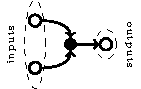
\includegraphics{example_open_graph_1}
\]
Whenever there is a bijection between the inputs of one graph and the outputs of another, we can connect them in a way described by the bijection.  This process is provides a way to turn a pair of compatible open graphs into a single open graph.  For instance, we cannot connect 
\[
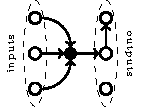
\includegraphics{example_open_graph_2}
\]
to the above open graph, though we can connect 
\[
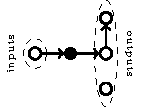
\includegraphics{example_open_graph_3}
\]
to form the open graph
\[
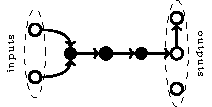
\includegraphics{example_open_graph_4}
\]

This is made precise using cospans and pushout as follows. Consider the functor $N \from \cat{Set}_0 \to \cat{Graph}$ on a skeleton of $\cat{Set}$ given by the letting $N(X)$ be the edgeless graph with nodes $X$.  An \emph{open graph} is then a cospan in the category $\cat{Graph}$ of the form $N(X) \to G \gets N(Y)$ for sets $X$ and $Y$. We will denote this open graph by $G$ when the legs of the cospan do not need to be explicit.  Also, call the left leg $N(X)$ of the cospan the \emph{inputs} of $G$ and the right leg $N(Y)$ the \emph{outputs} of $G$.  Suppose we have another open graph $G'$ with inputs $N(Y)$ and outputs $N(Z)$.  Then we can compose the cospans 
\[
N(X) \to G \gets N(Y) \to G' \gets N(Z). 
\] 
This is certainly not an open graph, but pushing out over the span $G \gets N(Y) \to G'$ induces the open graph  
\[
N(X) \to G +_{N(Y)} G' \gets N(Z).
\] 
By taking isomorphism classes of these pushouts, we obtain a category whose objects are those in the image of $N$ and morphisms are open graphs. 

But we can do better! Indeed, we have only just described the first layer of a symmetric monoidal and compact closed (SMCC) bicategory introduced by the author under the name $\cat{Rewrite}$ \cite{Cicala_SpansCospans}. It was shown that $\cat{Rewrite}$ is SMCC in a joint work with Courser \cite{CicalaCourser_BicatSpansCospan}. Before moving on to consider graphs equipped with some additional structure, we briefly recall the story of $\cat{Rewrite}$ so that we can replicate that work to our present needs.

Given a topos $\cat{C}$, there is a SMCC bicategory $\bimonspcsp{C}$ consisting of 
\begin{itemize}
	\item (0-cells) objects of $\cat{C}$,
	\item (1-cells) cospans in $\cat{C}$, and
	\item (2-cells) isomorphism classes of monic spans of cospans in $\cat{C}$.
\end{itemize} 
This bicategory is helpful to model graphical calculi, however, the monic leg requirement is too restrictive for our purposes. So, we instead use a SMCC bicategory $\bispcs{C}$, defined just as $\bimonspcsp{C}$ except with the $2$-cells weakened to morphism classes of spans of cospans in $\cat{C}$.  By morphism classes, we mean the equivalence relation generated by the relation defined as $S \sim S'$ if there is a morphism of spans of cospans $S \to S'$.  This can also be conceptualized as the isomorphism classes between spans of cospans in the groupoid generated by $\cat{C}$. Figure \ref{fig:spans of cospans} diagrams both types of $2$-cells and their morphisms.  In fact, with these larger classes of $2$-cells, we no longer require $\cat{C}$ to be a topos, though this plays no role currently.

\begin{figure}
	\fbox{%
	\begin{minipage}{\textwidth}
	\centering
	\subcaptionbox{$\bimonspcsp{C}$}[.3\textwidth]{%
		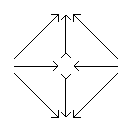
\includegraphics{diagram_monic_span_cospans}
	}
	~
	\subcaptionbox{$\bispcs{C}$}[.3\textwidth]{%
		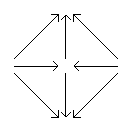
\includegraphics{diagram_span_cospans}
	}
	~
	\subcaptionbox{Morphism}[.3\textwidth]{%
	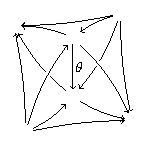
\includegraphics{(scC)+(Map_of_Spans_of_Cospans)}
	}
	\end{minipage}
}
\caption{Spans of cospans}
\label{fig:spans of cospans}
\end{figure}



Letting $\cat{C}$ be the category $\cat{Graph}$ of directed graphs, we defined the earlier mentioned SMCC bicategory $\cat{Rewrite}$ as the $1$-full and $2$-full sub-bicategory of $\bispcs{Graph}$ whose  $0$-cells are exactly the edgeless graphs. The concept of $\cat{Rewrite}$ is that the $1$-cells are open graphs and the $2$-cells are the rewritings of open graphs in a way that preserves the input and output nodes. By rewriting, we mean double pushout graph rewriting \cite{Corradini_AlgAppGraphTrans}.

The motivation for constructing $\cat{Rewrite}$ is not necessarily to study it directly, but rather for it to serve as an ambient context in which to generate SMCC sub-bicategories on some collection of open graphs and rewriting rules. Of course, the collection that one would use depends on their interest. For instance, if one were interested in topological quantum field theories, Courser and the author categorify $\cat{2Cob}$, the category of smooth compact $1$-dimensional manifolds without boundary and smooth compact oriented cobordisms \cite{CicalaCourser_BicatSpansCospan}.

The interest in $\cat{Rewrite}$ is that graphical calculi typically use some version of open graphs as a semantics and equations between graphical terms are given by rewrite rules \cite{Selinger_GraphicsMonCats}. However, equations are never as good as $2$-cells when when viewing through categorical lens.  Equations ought to be replaced by isomorphisms. The process of replacing equations with isomorphisms and sets by categories is known as categorification. In this program, we are interested in categorifying certain categories into bicategories. The categories of interest are those whose morphisms are associated to open graphs of some sort. For instance there are various categories of open networks \cite{Dixon_OpenGraphs,Fong_AlgOpenSystems,Pollard_OpenMarkov} which we seek to categorify by interpreting rewrite rules as $2$-cells instead of as providing equations between morphisms.  However, this requires some work.

There are drawbacks to this approach. For example, working with open graphs is only useful to model graphical calculi whose terms are equal up to ambient isotopy in $4$-space. Selinger's work \cite{Selinger_GraphicsMonCats} excellently describes various graphical calculi and the role ambient isotopy plays in their use. Amending $\cat{Rewrite}$ to account for this shortcoming is a direction of future research.  Currently, our interest lies in expanding the idea of $\cat{Rewrite}$ to categorify the zx-calculus.

%%%%%%%%%%%%%%%%%%%%%%
%%%%%%%%%%%%%%%%%%%%%%
% THE ZX-CALCULUS
\section{The zx-calculus}
\label{sec:ZxCalc}
%%%%%%%%%%%%%%%%%%%%%%
%%%%%%%%%%%%%%%%%%%%%%

One of the most fascinating features of quantum physics is the incompatibility of observables, which are, roughly, measurable quantities of some system.  Arguably, the most famous example of this is Heisenberg's uncertainty principal which places limits to the precision that one can simultaneously measure a pair of observables: position and momentum.  There are different levels of incompatibility amongst pairs of observables. When such a pair is maximally incompatible, in the sense that knowing the one with complete precision implies total uncertainty of the other, we say they are \emph{complementary observables}.  

The study of observables typically leads one to work in a Hilbert space, where a vector represents a state of the system. Even though this formalism has been incredibly fruitful, computations in Hilbert spaces can be difficult and non-intuitive. The zx-calculus was developed by Coecke and Duncan \cite{CoeckeDuncan_QuantumObs} as a high-level language to facilitate such computation.  At its core, the zx-calculus is an intuitive graphical language in which to reason about complementary observables. 

The five `generating elements' to the zx-calculus are depicted in Figure \ref{fig:ZX generators} and are to be read from left to right. They are
\begin{itemize}
	\item a wire with a single input and output,
	\item green \emph{spiders} with a non-negative integer number of inputs and outputs and paired with a phase $\alpha \in [-\pi,\pi)$,
	\item red \emph{spiders} with a non-negative integer number inputs and outputs and paired with a phase $\beta \in [-\pi,\pi)$,
	\item a yellow node with a single input and output, and
	\item a black diamond node with no inputs or outputs.
\end{itemize}
The wire plays the role of the identity, much like a plain wire in an electrical circuit, or straight pipe in a plumbing system. The green and red spiders arise from a pair of complementary observables.  It was determined that observables correspond to certain commutative Frobenius algebras $A$ living in a dagger symmetric monoidal category $\cat{C}$ \cite{CoeckePavlovic_QuantumMeasSums, CoeckePavVicary_OrthBasis}.  Frobenius algebras have nice representations as string diagrams which influenced the depiction of the spiders. Now, if $I$ is the monoidal unit of $\cat{C}$, there is an isomorphism $\cat{C}(I,A) \to \cat{C}(A,A)$ of commutative monoids which gives rise to a phase group on $A$.  It is from this that we get the phases on the spiders. The Hadamard node embodies the Hadamard gate. The diamond follows from the notion of `coherence', which exists between observable structures if certain equations are satisfied.  

In the spirit of compositionality, we will soon present a category $\cat{zx}$ whose morphisms are generated by these five diagrams, so we will go ahead and call them $\cat{zx}$-morphisms. In particular, we will call the five $\cat{zx}$-morphisms listed above as \emph{basic}.
\begin{figure}
	\fbox{%
		\begin{minipage}{\textwidth}
			\centering
			%%%%%%%%%%%%%%%%%%%%%%
			\subcaptionbox{Wire}[.1\textwidth]{%
				
\includegraphics{generater_wire}
			}
			~
			\subcaptionbox{Green spider}[.2\textwidth]{%
				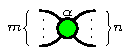
\includegraphics{generater_green_spider}
			}
			~
			\subcaptionbox{Red spider}[.2\textwidth]{%
				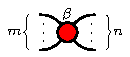
\includegraphics{generater_red_spider}
			}
			~
			\subcaptionbox{Hadamard}[.2\textwidth]{%
				
\includegraphics[]{generater_hadamard}
			}
			~
			\subcaptionbox{Diamond}[.15\textwidth]{%
				
\includegraphics{generater_diamond}
			}
			%%%%%%%%%%%%%%%%%%%%%%
		\end{minipage}
	}
	\caption{Generators for the category $\cat{zx}$}
	\label{fig:ZX generators}
\end{figure}

Observe that there is a non-negative number of dangling wires on the right and left sides of these basic $\cat{zx}$-morphisms. We will refer to those wires on the left as \emph{inputs} and those on the right as \emph{outputs}. With this in mind, we now present the dagger compact category $\cat{zx}$ introduced by Coecke and Duncan \cite{CoeckeDuncan_QuantumObs} and further studied by Backens \cite{Backens_Completeness}. The objects of $\cat{zx}$ are the non-negative integers.  The morphisms are generated by those depicted in Figure \ref{fig:ZX generators}, though we take the wire to be the identity on $1$.  Composition in $\cat{zx}$ is performed by separately enumerating the inputs and outputs of a pair of compatible diagrams  and connecting the outputs of the first diagram to the inputs of the second diagram along the enumeration.  The monoidal product on $\cat{zx}$ is given by addition on the objects and the disjoint union of diagrams on the morphisms. From this, we obtain the identity on all $n$ by taking the disjoint union of $n$ wires. The symmetry of the monoidal product gives us a morphism
\[

\includegraphics{morphism_zx_braiding}
\]
The compactness provides evaluation and coevaluation morphisms
\[
	\raisebox{-0.5\height}{%
		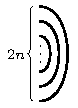
\includegraphics{morphism_zx_evaluation}
	}
	\quad \text{and} \quad
	\raisebox{-0.5\height}{%
		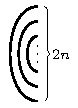
\includegraphics{morphism_zx_coevaluation}
	}
\]
from $2n \to 0$ and $0 \to 2n$ for each object $n \geq 1$ and the empty diagram for $n=0$.  The dagger structure is obtained by swapping inputs and outputs then, for the spider diagrams, multiplying the phase by $-1$.  For instance, 
\[
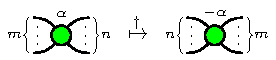
\includegraphics{functor_dagger}
\]
The dagger acts trivially on the wire, Hadamard, and diamond elements. 

\begin{figure}[h]
	\fbox{
		\begin{minipage}{\textwidth}
			\centering
			%%%%%%%%%%%%%%%%%%%%%%
			\begin{subfigure}[t]{0.4\textwidth}
				\centering
				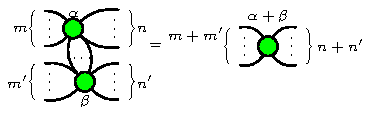
\includegraphics{equation_spider}
				\caption{Spider equation}
			\end{subfigure}%
			~
			\begin{subfigure}[t]{0.5\textwidth}
				\centering
				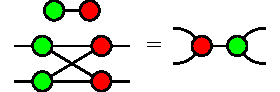
\includegraphics{equation_bialgebra}
				\caption{Bialgebra equation}
			\end{subfigure}%
			%%%%%%%%%%%%%%%%%%%%%%
			\vspace{2ex}
			%%%%%%%%%%%%%%%%%%%%%%
			
			\begin{subfigure}[t]{0.3\textwidth}
				\centering
				
\includegraphics{equation_cup}
				\caption{Cup equation}
			\end{subfigure}%
			~
			\begin{subfigure}[t]{0.3\textwidth}
				\centering
				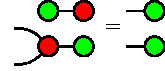
\includegraphics{equation_copy}
				\caption{Copy equation}
			\end{subfigure}%
			~
			\begin{subfigure}[t]{0.3\textwidth}
				\centering
				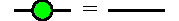
\includegraphics{equation_trivial_spider}
				\caption{Trivial spider equation}
			\end{subfigure}%
			%%%%%%%%%%%%%%%%%%%%%%
			\vspace{2ex}
			%%%%%%%%%%%%%%%%%%%%%%
			\begin{subfigure}[t]{0.33\textwidth}
				\centering
				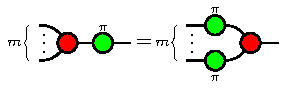
\includegraphics{equation_pi_copy}
				\caption{$\pi$-Copy equation}
			\end{subfigure}%
			~
			\begin{subfigure}[t]{0.33\textwidth}
				\centering
				
\includegraphics{equation_pi_commutation}
				\caption{$\pi$-Commutation equation}
			\end{subfigure}%
			~
			\begin{subfigure}[t]{0.33\textwidth}
				\centering
				
\includegraphics{equation_loop}
				\caption{Loop equation}
			\end{subfigure}%
			%%%%%%%%%%%%%%%%%%%%%%
			\vspace{2ex}
			%%%%%%%%%%%%%%%%%%%%%%
			\begin{subfigure}[t]{0.4\textwidth}
				\centering
				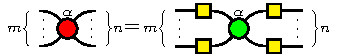
\includegraphics{equation_color_change}
				\caption{Color change equation}
			\end{subfigure}%
			~
			\begin{subfigure}[t]{0.4\textwidth}
				\centering
				
\includegraphics{equation_diamond}
				\caption{Diamond equation}
			\end{subfigure}%
			%%%%%%%%%%%%%%%%%%%%%%
		\end{minipage}
	}
	\caption{Relations in the category $\cat{zx}$}
	\label{fig:ZX equations}
\end{figure}

 
Thus far, we have a presentation for a free dagger compact category. However, there are many relations that hold between diagrams.  The emergence of these relations is technical and the interested reader should read about the genesis of the zx-calculus \cite{CoeckeDuncan_QuantumObs} to learn the story. These generating relations of $\cat{zx}$ are depicted in Figure \ref{fig:ZX equations}, though we add equations to that list obtained by 
\begin{itemize}
	\item by exchanging red and green nodes, 
	\item by daggering, and
	\item up to ambient isotopy in $4$-space.
\end{itemize}
These listed relations will be called \emph{basic}. Note that we denote the empty graph, which is the monoidal unit, by $\emptyset$. Also, red and green nodes with no phase indicated have a phase of $0$. 

%%%%%%%%%%%%%%%%%%%%%%
%%%%%%%%%%%%%%%%%%%%%%
% OPEN STRUCTURED GRAPHS
\section{Open graphs over $S\zx$}
\label{sec:OpenGraphsOverSzx}
%%%%%%%%%%%%%%%%%%%%%%
%%%%%%%%%%%%%%%%%%%%%%

In Section \ref{sec:RewritingOpenGraphs}, we saw that there is a SMCC bicategory $\bispcs{C}$. In particular, we discussed the SMCC sub-bicategory $\cat{Rewrite}$ of $\bispcs{Graph}$.  However, the $\cat{zx}$-morphisms are like graphs with additional structure, $\cat{Rewrite}$ is not enough to model the zx-calculus.  We need some new construction, analogous to $\cat{Rewrite}$, that works with open graphs with this additional structure. In this section, we determine exactly what structure is needed and produce the desired SMCC bicategory $\cat{zxRewrite}$. 

Let $S$ be a graph.  By a \emph{graph over $S$}, we mean a graph morphism $G \to S$. Then a morphism between graphs over $S$ is a graph morphism $G \to G'$ such that 
\[
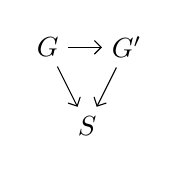
\begin{tikzpicture}
\node (1) at (-0.5,1) {$G$};
\node (2) at (0.5,1) {$G'$};
\node (3) at (0,0) {$S$};
%
\path[->,font=\scriptsize,>=angle 90]
(1) edge (2)
(1) edge (3)
(2) edge (3);
\end{tikzpicture}
\]
The additional structure we seek to put are graphs is done by simply working with graphs over $S$ instead of graphs. Specifically,  $G$ absorbs the structure of $S$ via the fibres of the morphism. We illustrate this with the following example.

\begin{ex}
\label{ex:basic graph over Szx}
	Let $S_{\text{zx}}$ be the graph
\begin{equation}
\label{diag:zx struture graph}
\raisebox{-0.75\height}{
	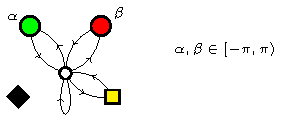
\includegraphics{graph_S_zx}
}
\end{equation}

We have not drawn the entirety of $S_{\text{zx}}$. Actually, the green and red nodes run through $[-\pi,\pi)$ and all of them have a single arrow to and from node 
$

\begin{tikzpicture}
	\node [zxopen] at (0,0) {};
\end{tikzpicture}
$. 

We can capture much of the structure of the basic $\cat{zx}$-morphisms in Figure \ref{fig:ZX generators} as graphs over $S_{\text{zx}}$:
\[
	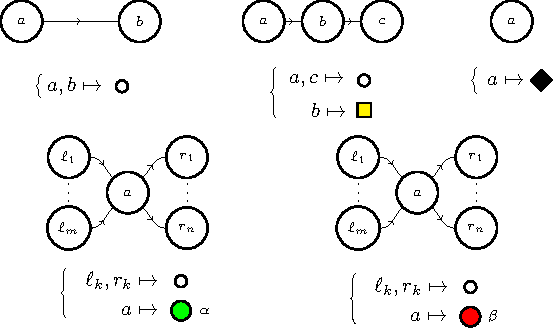
\includegraphics{graph_over_Szx}
\]
Note that the functions are completely determined by their behavior on the nodes because there is at most one arrow between any two nodes in $S_{\text{zx}}$.  The role each of the nodes in $S_{\text{zx}}$ plays in providing structure is evident except, perhaps, for the node
$

\begin{tikzpicture}
\node [zxopen] at (0,0) {};
\end{tikzpicture}
$.   
Observe that four of the basic zx-elements have dangling wires on either end.  Because edges of directed graphs must be attached to a pair of nodes, we use this node to anchor the dangling edges.
\end{ex}

\begin{ex}
\label{ex:graph over Szx}
At this point, we can think of the basic elements of the zx-calculus as graphs over $S_{\text{zx}}$. But we can actually do this for any $\cat{zx}$-morphism, such as
\[
	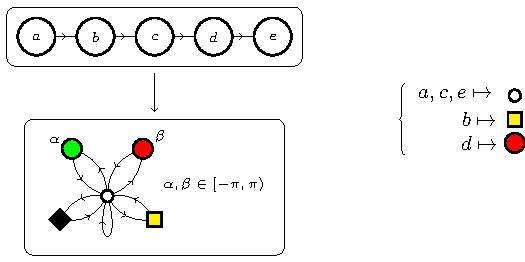
\includegraphics{example_graph_over_Szx}
\]
This corresponds with the $\cat{zx}$-morphism 
\[
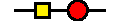
\includegraphics{example_zx_morphism_as_graph_over_Szx}
\]
\end{ex}

Above, we mentioned that the graphs over $S\zx$ in Example \ref{ex:basic graph over Szx} capture ``most" of the structure of the basic $\cat{zx}$-morphisms.  the difference is, with the basic $\cat{zx}$-morphisms, we are able to compose. Therefore, if we aim to describe $\cat{zx}$-morphisms with graphs over $S\zx$, we need to be able to connect graphs over $S_{\text{zx}}$ in a way that captures composition. A way to accomplish this is to equip graphs over $S_{\text{zx}}$ with inputs and outputs as we did for open graphs.  Again, we use cospans, though the added structure introduces new considerations. 

Consider the over category $\zxGraphs$ of graphs over $S_{\text{zx}}$. As discussed earlier, this gives us an SMCC bicategory $\cat{Sp}(\cat{Csp}(\cat{Graph}\downarrow S_{\text{zx}}))$.  Now, we would like to construct a sub-bicategory in a similar vein to $\cat{Rewrite}$.  However, there is a problem.  Recall that the objects of $\cat{Rewrite}$ have the form $N(X)$ where $N \from \cat{Set}_0 \to \cat{Graph}$ is the functor sending a set to the edgeless graph on that set.  In $\cat{Graph}$, there is a unique way to be an edgeless graph. But in $\zxGraphs$ there is not a unique (up to isomorphism) way to be an edgeless graph because there may be more than one graph morphism to $S_{\text{zx}}$. For instance, the graph with two nodes and no edges can be a graph over $S_{\text{zx}}$ in $5^2 = 25$ ways. This issue is rectified by functorially choosing which edgeless graphs over $S_{\text{zx}}$ will serve as inputs and outputs. This lets us expand the notion of graphs over $S_{\text{zx}}$ to `open graphs over $S_{\text{zx}}$'.  

\begin{defn}
	Define a functor 
	\[
		N_{\text{zx}} \from \cat{Set}_0 \to \zxGraphs
	\] 
	by $X \mapsto (N_{\text{zx}}(X) \to S_{\text{zx}})$ where $N_{\text{zx}}(X)$ is the edgeless graph with nodes $X$ and each node is mapped to $
\begin{tikzpicture} \node [zxopen] at (0,0) {}; \end{tikzpicture}$. 
An \emph{open graph over $S_{\text{zx}}$} is a cospan in $\zxGraphs$ of the form
	\[
		N_{\text{zx}}(X) \to G \gets N_{\text{zx}} (Y).
	\]
\end{defn}

At this point, we are ready to define the analogue to $\cat{Rewrite}$. 

\begin{defn}
	Define a bicategory $\cat{zxRewrite}$ as the symmetric monoidal and compact closed sub-bicategory of $\SpCspZX$ that is $1$-full and $2$-full on the objects of the form $N\zx (X)$ for sets $X$.  
\end{defn}

The $0$-cells of $\cat{zxRewrite}$ are those edgeless graphs over $S\zx$ in the image of $N\zx$.  The $1$-cells are exactly the open graphs over $S\zx$. The $2$-cells are all the ways to rewrite one open graph over $S\zx$ into another in a way that preserves the inputs and outputs.  

To better understand this bicategory, we give an example of an open graph over $S_{\text{zx}}$. Along with this example, we introduce new notation in order to keep the remaining diagrams rather compact. This notation includes the information of an open graph $G \to S\zx$ completely in the nodes of $G$ by drawing each node of $G$ in the same way as its image is drawn in $S_{\text{zx}}$. Moreover, the legs of the cospans have associated cardinalities $\kappa$ and $\kappa'$ which we will write in the lower left and right corners of the graph.  The following example should clarify this notation.

\begin{ex}
\label{ex:open graph over Szx}
Consider the graph over $S_{\text{zx}}$ in Example \eqref{ex:graph over Szx}.  Make this an open graph as follows:
\[
	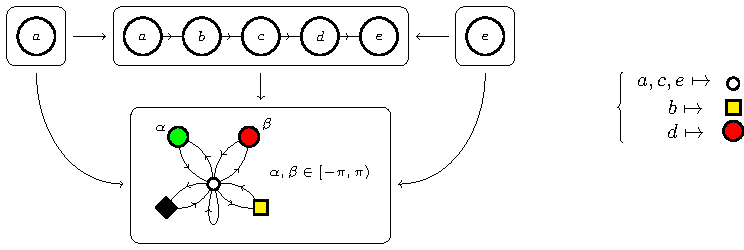
\includegraphics{example_open_graph_over_Szx}
\]
There is a single input, node $a$, and a single output, node $e$. Denote this by
\[
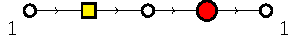
\includegraphics{example_zx_morphism_as_open_graph_over_Szx}
\]
Of course, this notation sheds away a fair amount information regarding the graph morphisms involved in the cospan. To gain a bit of the information back, we will align all input nodes on the far left and the output nodes on the far right. Assume that the left and right hand cospan maps are in bijection with these input nodes and output nodes, respectively. This should cause no confusion for our purposes here.
\end{ex}

As mentioned earlier, our interest in the category $\cat{Rewrite}$ is as an ambient context in which to generate symmetric monoidal and compact closed bicategories from some collection of $1$-cells and $2$-cells. The same can be said for our new bicategory $\cat{zxRewrite}$.  In particular, we want to have $1$-cells that correspond to the basic $\cat{zx}$-morphisms from Figure \ref{fig:ZX generators} and $2$-cells that correspond to the basic relations from Figure \ref{fig:ZX equations}.  Our claim is that the resulting bicategory categorifies the category $\cat{zx}$.

%%%%%%%%%%%%%%%%%%%%%%
%%%%%%%%%%%%%%%%%%%%%%
% ZX CATEGORIFIED
\section{A categorification of $\cat{zx}$}
\label{sec:zx categorified}
%%%%%%%%%%%%%%%%%%%%%%
%%%%%%%%%%%%%%%%%%%%%%

The basic $\cat{zx}$-morphisms in Figure \ref{fig:ZX generators} are naturally presented as open graphs over $S_{\text{zx}}$ as shown in Figure \ref{fig:ZX 1cells generators}.  At first glance, there seems to be a redundancy in the green and red spiders: $m$ and $n$ have each been written twice.  However, this is because each instance of $m$ and $n$ have different meanings.  The $m$ and $n$ written beside the brackets counts the number of nodes.  The $m$ and $n$ underneath the diagrams indicate how many nodes are in the edgeless graphs in the left and right legs, respectively, of the cospan the diagram represents.  We are not requiring the cospan maps to be injective even though this happens to be the case for our generators. 

\begin{figure}[h]
	\fbox{%
		\begin{minipage}{\textwidth}
			\centering
			%%%%%%%%%%%%%%%%%%%%%%
			\subcaptionbox{Wire}[.30\textwidth]{%
				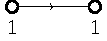
\includegraphics{1cell_zx_wire}
			}
			~
			\subcaptionbox{Hadamard}[.30\textwidth]{%
				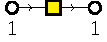
\includegraphics[]{1cell_zx_hadamard}
			}
			~
			\subcaptionbox{Diamond}[.30\textwidth]{%
				
\includegraphics{1cell_zx_diamond}
			}
			\linebreak
			\subcaptionbox{Green spider}[.4\textwidth]{%
				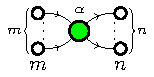
\includegraphics{1cell_zx_green_spider}
			}
			~
			\subcaptionbox{Red spider}[.4\textwidth]{%
				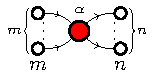
\includegraphics{1cell_zx_red_spider}
			}
			%%%%%%%%%%%%%%%%%%%%%%
		\end{minipage}
	}
	\caption{Generating $1$-cells for the bicategory $\bicat{zx}$}
	\label{fig:ZX 1cells generators}
\end{figure} 


Just as the open graphs over $S_{\text{zx}}$ in Figure \ref{fig:ZX 1cells generators} capture the generating $\cat{zx}$-morphisms, we also want to introduce the relations from Figure \ref{fig:ZX equations} into our framework.  These relations are presented in Figure \ref{fig:ZX 2cells generators}. There is an important difference between $\cat{zx}$ and our categorification $\bicat{zx}$ of it.  Namely, the wire is an identity in $\cat{zx}$, though not in $\bicat{zx}$.  To ensure that the wire behaves as we would like in $\bicat{zx}$, we include $2$-cells beyond those shown in Figure \ref{fig:ZX 2cells generators}. 

\begin{figure}[h]
	\fbox{%
		\begin{minipage}{\textwidth}
			\centering
			%%%%%%%%%%%%%%%%%%%%%%
			\subcaptionbox{Spider}[\textwidth]{%
				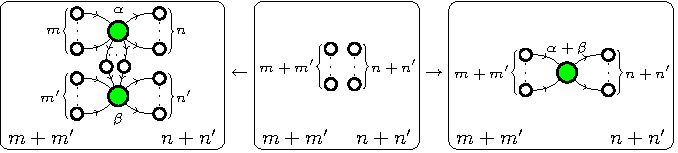
\includegraphics[scale=1]{2cell_spider}
			}
			\linebreak
			\subcaptionbox{Bialgebra}[\textwidth]{%
				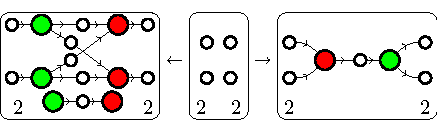
\includegraphics[scale=1]{2cell_bialgebra}
			}
			\linebreak
			\subcaptionbox{Cup}[0.45\textwidth]{%
				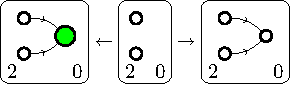
\includegraphics[scale=1]{2cell_cup}
			}
			\subcaptionbox{Copy}[0.45\textwidth]{%
				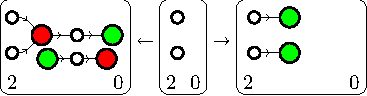
\includegraphics[scale=1]{2cell_copy}
			}
			\linebreak
			\subcaptionbox{Trivial spider}[0.45\textwidth]{%
				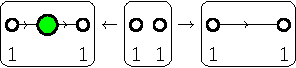
\includegraphics[scale=1]{2cell_trivial_spider}
			}
			\linebreak
			\subcaptionbox{$\pi$-copy}[0.45\textwidth]{%
				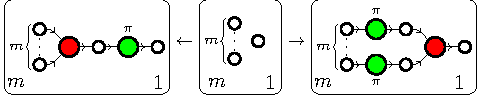
\includegraphics[scale=1]{2cell_pi_copy}
			}
			\linebreak
			\subcaptionbox{$\pi$-commutation}[\textwidth]{%
				\includegraphics[scale=1]{2cell_pi_commutation}
			}
			\linebreak
			\subcaptionbox{Color change}[\textwidth]{%
				\includegraphics[scale=1]{2cell_color_change}
			}
			\linebreak
			\subcaptionbox{Loop}[0.45\textwidth]{%
				\includegraphics[scale=1]{2cell_loop}
			}
			\subcaptionbox{Diamond}[0.45\textwidth]{%
				\includegraphics[scale=1]{2cell_diamond}
			}
			%%%%%%%%%%%%%%%%%%%%%%
		\end{minipage}
	}
	\caption{Generating $2$-cells for the bicategory $\bicat{zx}$}
	\label{fig:ZX 2cells generators}
\end{figure}

\begin{defn}
	\label{def:zx bicat}
	Define $\bicat{zx}$ to be the symmetric monoidal and compact closed sub-bicategory of $\cat{zxRewrite}$ generated by the $1$-cells depicted in Figure \ref{fig:ZX 1cells generators}.  The $2$-cells are generated by those spans of spans Figure \ref{fig:ZX 2cells generators}.  In addition, we also include $2$-cells obtained by exchanging red and green nodes, swapping inputs and outputs for each graph over $S\zx$, or by turning the spans around.  There is also an additional $2$-cell
	\[
		\includegraphics{2cell_wire_is_identity}
	\]
	added to account for the fact that the wire $1$-cell is not the identity on $1$ here. With the inclusion of this $2$-cell, we can replace a wire with an identity.
\end{defn}

Because $\bicat{zx}$ is symmetric monoidal and compact closed, it also contains a twist $1$-cell, plus evaluation and coevaluation $1$-cells for the compact structure on $m$ 
\begin{equation}
\label{diag:TwistCompact 1cells}
\raisebox{-1\height}{
	\includegraphics{1cell_zx_braiding}
	\quad \quad \quad
	\includegraphics{1cell_zx_evaluation}
	\quad \quad \quad
	\includegraphics{1cell_zx_coevaluation}
}
\end{equation}

There are two ways to make the new $1$-cells from old in $\bicat{zx}$: composing and tensoring.  Composing, of course, is made precise with pushouts. For example, we can compose the red and green spider diagrams
\[
\includegraphics{example_composable_spiders}
\]
only when $n=m'$.  In that case the composite $1$-cell is 
\[
	\includegraphics{example_composed_spiders}
\]
Tensoring $1$-cells is simply a matter of taking the disjoint union, as seen here: 
\[
	\includegraphics{diagram_tensor_spiders}
\]

Because $\bicat{zx}$ is a bicategory, $2$-cells are closed under vertical and horizontal composition, a detailed account of which was presented while originally defining $\cat{Rewrite}$ \cite{Cic}.  Instead of rehashing this, we provide a brief example to illustrate each composition. To clarify the situation, we will not use the notation introduced above and instead depict the spans and cospans in the $2$-cells. The graph morphisms involved are the monomorphism indicated by the placement of the nodes.  Vertical composition is performed by pulling back the cospan through the middle graph, as seen here:
\[
	\includegraphics[scale=0.75]{example_vertical_composition}
\]
Horizontal composition is performed by pushing out over each of the three spans through the middle graph. For instance
\[
	\includegraphics[scale=0.75]{example_horizontal_composition}
\]
Having defined $\bicat{zx}$, we can turn our focus towards presenting the main theorem showing that it categorifies $\cat{zx}$. We start with the following definition.

\begin{defn}
	Define $\operatorname{decat}(\bicat{zx})$ to be the category whose objects are the $0$-cells of $\bicat{zx}$ and whose arrows the $1$-cells of $\bicat{zx}$ modulo the equivalence relation $\sim$ given by 
	\begin{center}
		$f \sim g$ if and only if there is a $2$-cell $f \Rightarrow g$ in $\bicat{zx}$.
	\end{center}
\end{defn}

Just to be clear, the above actually is an equivalence relation and doesn't merely generate one.  This follows from the symmetric of spans and vertical composition.   

\begin{lem}
	The category $\operatorname{decat}(\bicat{zx})$ is dagger compact via the identity on objects functor described by 
	\[
	\raisebox{-0.5\height}{%
	\includegraphics{functor_dagger_decat_zx_spider_green}
	}
	\quad \text{and} \quad
	\raisebox{-0.5\height}{%
	\includegraphics{functor_dagger_decat_zx_spider_red}
	}
	\]
	as well as by identity on the wire, Hadamard, and diamond morphisms.
\end{lem}
\begin{proof}
	The category is compact closed because the objects are self dual with the evaluation maps and coevaluation maps from \eqref{diag:TwistCompact 1cells}.  Moreover, we can derive the snake equation
	\[
		\includegraphics{equation_decat_zx_snake}
	\]
	where the equalities follow from the evident $2$-cells in $\bicat{zx}$. The extra relation introduced in Definition \ref{def:zx bicat} ensures the string of wires is the identity. 
	
	 Showing that the described functor is a dagger functor is a matter of checking some easy to verify details. For instance, $\dagger$ behaves as required on the compact evaluation and coevaluation maps by recognizing that those can be drawn
	\[
	\raisebox{-0.5\height}{
	\includegraphics{morphism_decat_zx_dagger_on_evaluation}
	}
	\quad \text{and} \quad 	
	\raisebox{-0.5\height}{
	\includegraphics{morphism_decat_zx_dagger_on_coevaluation}
	}
	\qedhere
	\]
\end{proof}


\begin{thm}
\label{thm:equiv of zx cats}
	The identity on objects, dagger compact functor given by
	\[
		E \from \cat{zx} \to \operatorname{decat}(\bicat{zx})
	\]
	\begin{minipage}{0.5\textwidth}
	\begin{align*}
	\raisebox{-0.4\height}{\includegraphics{generater_green_spider} }
		& \mapsto
		\raisebox{-0.55\height}{\includegraphics{1cell_zx_green_spider}} \\
	& \\
	\raisebox{-0.45\height}{\includegraphics{generater_wire}}
		& \mapsto
		\raisebox{-0.65\height}{\includegraphics{1cell_zx_wire}}
	\end{align*}
	\end{minipage}
	\begin{minipage}{0.5\textwidth}
		\begin{align*}
		\raisebox{-0.35\height}{\includegraphics{generater_red_spider}}
			& \mapsto
			\raisebox{-0.55\height}{\includegraphics{1cell_zx_red_spider}} \\
		& \\
		\raisebox{-0.2\height}{\includegraphics{generater_hadamard}}
			& \mapsto
			\raisebox{-0.65\height}{\includegraphics{1cell_zx_hadamard}}
		\end{align*}
	\end{minipage}
	\[
	\raisebox{-0.3\height}{\includegraphics{generater_diamond}}
	\mapsto
	\raisebox{-0.65\height}{\includegraphics{1cell_zx_diamond}}
	\]
	is an equivalence of categories.
\end{thm}
\begin{proof}
	Essential surjectivity follows immediately from $E$ being identity on objects.  Fullness follows from the fact that the morphism generators for $\operatorname{decat}(\bicat{zx})$ are all in the image of $E$. 
	
	Faithfulness is more involved. Let $f,g$ be $\cat{zx}$-morphisms. Let $\widetilde{Ef}$, $\widetilde{Eg}$ be the representatives of $Ef$, $Eg$ obtained by directly translating the graphical representation of $f,g$ to open graphs of $S\zx$ as in Examples \ref{ex:graph over Szx}  and \ref{ex:open graph over Szx}. We claim that the existence of a $2$-cell $\widetilde{Ef} \Rightarrow \widetilde{Eg}$ in $\bicat{zx}$ implies that $f=g$.  Showing this claim implies that $E$ is faithful. 
	
	Observe that any $2$-cell $\alpha$ can be written, not necessarily uniquely, as sequence $\alpha_1 \square \dotsm \square \alpha_n$ of length $n$ where each $\alpha_i$ is one of the basic $2$-cells and each `$\square$' is filled in with either `$\circ_\t{h}$', `$\circ_\t{v}$', or `$+$' and parenthesis are right justified. By `$\circ_\t{h}$' and `$\circ_\t{v}$', we mean horizontal and vertical composition. We will induct sequence length.  If $\alpha \from \widetilde{Ef} \Rightarrow \widetilde{Eg}$ is a basic $2$-cell, then there is clearly a corresponding basic relation equating $f$ and $g$.  Suppose that our claim holds for any $2$-cell that can be written as a length $n$ sequence.  Then there are three ways to be a length $n+1$ sequence, one for each possible way one of the three operations can fill the left-most square.  If the left-most square is a $'+'$, then we have a $2$-cell $\alpha_1 + \alpha_2 \from Ef \Rightarrow Eg$ where $\alpha_1$ is a basic $2$-cell and $\alpha_2$ can be written with length $n$.   By fullness, we can write $\alpha_1 + \alpha_2 \from Ef_1 + EF_2 \Rightarrow Eg_1 + Eg_2$ where $\alpha_i \from Ef_i + Eg_i$.   This gives that $f_i = g_i$  and the result follows.  A similar argument handles the cases when the left-most operation is vertical or horizontal composition.
\end{proof}

%%%%%%%%%%%%%%%%%%%%%%
% APPENDIX
\appendix
\label{sec:appendix}
%%%%%%%%%%%%%%%%%%%%%%

Suppose that $\cat{C} \coloneqq (\cat{C}_0, \otimes, I)$ is a symmetric monoidal category.  Using Shulman's work \cite{Shul}, we will show that $\cat{cs}(\cat{C})$ is a (symmetric, braided) monoidal category. We will not cover the details of Shulman's work here.  The main point we will use, however, is the following theorem.

\begin{thm}[{\cite[{Thm.~1.2}]{Shul}}]
	\label{thm:Shulmans thm}
	The underlying bicategory of an isofibrant symmetric monoidal double category is symmetric monoidal.  
\end{thm}

Roughly, a \emph{double category} $\DD$ consists of an object category $\DD_\t{ob}$ and arrow category $\DD_\t{ar}$ along with structure functors satisfying certain equations:
\begin{itemize}
	\item $U \from \DD_\t{ob} \to \DD_\t{ar}$ picking out identities,
	\item $S,T \from \DD_\t{ar} \to \DD_\t{ob}$ picking out sources and targets, and
	\item $\odot \from \DD_\t{ar} \times_{\DD_\t{ob}} \DD_\t{ar} \to \DD_\t{ar}$ giving the composition, with the pull back taken over $S$ and $T$.
\end{itemize}
There are also functors realizing associativity plus left and right unity satisfying several properties and coherence axioms.  This can be depicted by
\[
\includegraphics{(Double_Cat)+(2Cell_General_Form)}
\]
where the bullets are $\DD_\t{ob}$-objects, $f,g$ are $\DD_\t{ob}$-morphisms, $M,N$ are $\DD_\t{ar}$-objects, and $a$ is a $\DD_\t{ar}$-morphism.  In case $f$ and $g$ are identities, we say that $a$ is \emph{globular}.

There is a lot to unpack from the definition of a symmetric monoidal double category $\DD = (\DD_0,\otimes,I)$, and we will point the interested reader again to Shulman \cite[Def.~2.9]{Shul}.  The underlying bicategory of $\DD$ is given by
\begin{itemize}
	\item ($0$-cells) $\DD_\t{ob}$-objects,
	\item ($1$-cells) $\DD_\t{ar}$-objects, and
	\item ($2$-cells) globular $\DD_\t{ar}$-morphisms.
\end{itemize}
Also, we say that $\DD$ is \emph{isofibrant} if, for every $\DD_\t{ob}$-morphism $f$, there is a  $\DD_\t{ar}$-object $f'$ together with $\DD_\t{ar}$-morphisms
\[
\includegraphics[]{(Double_Cat)+(Companion_2Cells)}
\]
that satisfy the equations
\[
\includegraphics[]{(Double_Cat)+(Companion_Equations)}
\]

Now that we know what how to interpret the above theorem, we will construct a double category satisfying the necessary hypothesis. Let $\cat{cs}(\CC)$ be the double category given by the categories 
\[
\cat{cs}(\CC)_\t{ob} \coloneqq \cat{Span}(\cat{C})
\] 
where $\cat{Span}(\cat{C})$ is the $1$-category of spans in $\cat{C}$, and also by
\[
\cat{cs}(\CC)_\t{ar}
\]
whose objects are $\cat{C}$-cospans and morphisms are spans of $\cat{C}$-cospans up to morphism. A morphism in $(\CC)_\t{ar}$ between cospans $a \to b \gets c$ and $a'' \to b'' \gets c''$ is a diagram
\begin{equation}
\label{eq:2morphism csCC generic}
\includegraphics[]{(csCC)+(2Morphism_General_Form)}
\end{equation}
in $\cat{C}$ up to morphism, by which we mean the obvious extension of notion of span of cospans up to morphism discussed earlier.  The functor $U \from \cat{cs}(\CC)\t{ob} \to \cat{cs}(\CC)\t{ar}$ sends a object to the identity cospan on it and sends a morphism $x \to y \gets z$ to 
\[
\includegraphics[]{(csCC)+(Identity_Functor_U)}
\]
The source functor $S \from \cat{cs}(\CC)_\t{ar} \to \cat{cs}(\CC)_\t{ob}$ sends a object $x \to y \gets z$ to $x$ and a morphism, say \eqref{eq:2morphism csCC generic}, to $x' \to y' \gets z'$.  Define the target functor $T$ similarly.  The composition functor $\odot \from \DD_\t{ar} \times_{\DD_\t{ob}} \DD_\t{ar} \to \DD_\t{ar}$ is more complicated.  We can illustrate its behavior by
\[
\includegraphics[]{(csCC)+(Composition_Functor)}
\]
Then to see whether $\odot$ preserves composition $\circ$, we need to show that 
\begin{equation}
\label{eq:Interchange Law for scCC}
(\alpha \odot \beta) \circ (\alpha' \odot \beta') = (\alpha \circ \beta) \odot (\alpha' \circ \beta'),
\end{equation} 
where
\[
\includegraphics[]{(scCC)+(Alpha_2cell)}
\quad
\includegraphics[]{(scCC)_(Alpha_Prime_2Cell)}
\]
\[
\includegraphics[]{(scCC)+(Beta_2Cell)}
\quad
\includegraphics[]{(scCC)+(Beta_Prime_2Cell)}
\]
First, we compute the left hand side of \eqref{eq:Interchange Law for scCC}, which corresponds with horizontal composition before vertical composition. 



%%%%%%%%%%%%%%%%%%%%%%%%%%%%%%%%%%%%%%%
%%%%%%%%%%%%%%%%%%%%%%%%%%%%%%%%%%%%%%%
%
% BIBLIOGRAPHY
%
%%%%%%%%%%%%%%%%%%%%%%%%%%%%%%%%%%%%%%%
%%%%%%%%%%%%%%%%%%%%%%%%%%%%%%%%%%%%%%%

\begin{thebibliography}{100}	
	%
	\bibitem{AbramCoecke_CatSemanticQuantum}
	S.~Abramsky and B.~Coecke, B. 
	(July 2004).
	\emph{A categorical semantics of quantum protocols}. 
	In Logic in Computer Science. 
	Proceedings of the 19th Annual IEEE Symposium on (pp. 415-425). IEEE.
	Chicago	
	%
	\bibitem{Backens_Completeness}
	M.~Backens.
	(2016). 
	\emph{Completeness and the ZX-calculus.} 
	Available as \href{https://arxiv.org/abs/1602.08954}{arXiv:1602.08954}.
	%
	\bibitem{Cicala_SpansCospans} 
	D.~Cicala.
	(2016). 
	\emph{Spans of cospans}.
	Available as \href{https://arxiv.org/abs/1611.07886}{arXiv:1611.07886}.
	%
	\bibitem{CicalaCourser_BicatSpansCospan}
	D.~Cicala and K.~Courser.
	\emph{Bicategories of spans and cospans}.
	In preparation.
	%
	\bibitem{CoeckeDuncan_QuantumObs}
	B.~Coecke and R.~Duncan. 
	(2011). 
	\emph{Interacting quantum observables: categorical algebra and diagrammatics}. 
	New Journal of Physics, 13(4), 043016.
	%
	\bibitem{CoeckePavlovic_QuantumMeasSums}
	B.~Coecke and D.~Pavlovic. 
	\emph{Quantum measurements without sums}. 
	Available as \href{https://arxiv.org/abs/quant-ph/0608035}{arXiv:quant-ph/0608035}.
	%
	\bibitem{CoeckePavVicary_OrthBasis}
	B.~Coecke, D.~Pavlovic, \& J.~Vicary. 
	(2013).
	\emph{A new description of orthogonal bases.} 
	Mathematical Structures in Computer Science, 23(03), pp.~555-567.
	%
	\bibitem{Corradini_AlgAppGraphTrans}
	A.~Corradini, U.~Montanari, F.~Rossi, H.~Ehrig, R.~Heckel, \& M.~L\"{o}we.
	(February 1997).
	\emph{Algebraic Approaches to Graph Transformation-Part I: Basic Concepts and Double Pushout Approach}. 
	In Handbook of Graph Grammars, pp.~163-246.
	%
	\bibitem{Dixon_OpenGraphs}
	L.~Dixon, R.~Duncan, and A.~Kissinger. 
	(2010).
	\emph{Open graphs and computational reasoning}. 
	Available as \href{https://arxiv.org/abs/1007.3794}{arXiv:1007.3794}.
	%
	\bibitem{Fong_AlgOpenSystems}
	B.~Fong. 
	(2016).
	\emph{The Algebra of Open and Interconnected Systems}. 
	Available as \href{https://arxiv.org/abs/arXiv:1609.05382}{arXiv:1609.05382}. 
	%
	\bibitem{JoyalStreet_GeomTensorCalc}
	A.~Joyal and R.~Street.
	(1991).
	 \emph{The geometry of tensor calculus, I}. 
	 Advances in Mathematics 88(1), pp.~55-112.
	 Also available at \href{http://www.sciencedirect.com/science/article/pii/000187089190003P}{http://www.sciencedirect.com/science/article/pii/000187089190003P}.
	%
	%\bibitem{MaclaneMoer}
	%S.~MacLane, and I.~Moerdijk. 
	%(2012).
	%\emph{Sheaves in Geometry and Logic: A First Introduction to Topos Theory}. 
	%Springer Science \& Business Media. 
	%
	\bibitem{Penrose_NegDimTensors}
	R.~Penrose. 
	(1971).
	\emph{Applications of negative dimensional tensors.} 
	Combinatorial mathematics and its applications.  221244.  
	Also available at \href{http://homepages.math.uic.edu/~kauffman/Penrose.pdf}{http://homepages.math.uic.edu/~kauffman/Penrose.pdf}
	%
	\bibitem{Pollard_OpenMarkov}
	B.~Pollard. 
	(2016).
	\emph{Open Markov processes: A compositional perspective on non-equilibrium steady states in biology}. Entropy, 18(4), pp.~140. 
	%
	\bibitem{Selinger_GraphicsMonCats}
	P.~Selinger. 
	(2010).
	\emph{A survey of graphical languages for monoidal categories}. 
	New Structures for Physics, pp. ~289-355. Springer Berlin Heidelberg. 
\end{thebibliography}


%%%%%%%%%%%%%%%%%%%%%%%%%%%%%%%%%%%%%%%
%%%%%%%%%%%%%%%%%%%%%%%%%%%%%%%%%%%%%%%
%%%%%%%%%%%%%%%%%%%%%%%%%%%%%%%%%%%%%%%
%
% END DOCUMENT
%
%%%%%%%%%%%%%%%%%%%%%%%%%%%%%%%%%%%%%%%
%%%%%%%%%%%%%%%%%%%%%%%%%%%%%%%%%%%%%%%
%%%%%%%%%%%%%%%%%%%%%%%%%%%%%%%%%%%%%%%
%%%%%%%%%%%%%%%%%%%%%%%%%%%%%%%%%%%%%%%

\end{document}